\chapter{Backup und Recovery}\label{cha:backup}

Es können viele Dinge passieren, die die Daten in einer Datenbank gefährden - Ausfälle, Fehlbenutzungen, etc. Gegenüber diesen Vorkommnissen muss man sich absichern.

\section{Arten von Backups}

\subsection{Physisches Backup}

Ein Physisches Backup kann hot/cold und Full/Incremental sein.
Dabei werden ganze Datenbankfiles auf Betriebssystemebene kopiert.
Physische Backups und Recoveries können mit dem RMAN-Tool durchgeführt werden.
RMAN unterstützt Inkrementelle Backups, speichert also nur geänderte Datenblöcke und hat einen speziellen Kompressionsalgorithmus, welcher für Oracle-DBs entwickelt wurde.
Man kann die Backups mit ihm verschlüsseln. RMAN hat viele Optimierungen, wie z.B dass beim Recovery nicht betroffene Blöcke übersprungen werden können.

\subsection{Physisches Hot Backup}

Während des Backups können Benutzer das System verwenden. Die Changes die während des Backups passieren werden separat mitgelogged, und dann auf das Backup vorwärtsgerollt. (Rolling Forward = REDO-Log-Files anwenden - im vergleich zu Rolling Back = REDO-Logs rückwärts abspielen). Hierbei ist die Gefahr, dass Backup und DB nicht zur Gänze synchronisiert sind.

\subsection{Physisches Cold backup}

Kopieren passiert während die DB gerade in Downtime - also nicht für User zugänglich, bzw. heruntergefahren - ist.

\subsection{Physisches Inkrementelles Backup}

Hierbei werden nur Änderungen (REDO-Log-Files) kopiert, die seit dem letzten Backup passiert sind. Ein Vorteil ist, dass ein Inkrementelles Backup Hot gemacht werden kann, ohne eine große Auswirkung auf die Nutzer zu haben (DB wird nur etwas langsamer).

\subsection{Physisches Full Backup}

Hierbei wird die ganze Datenbank kopiert. Dies sollte Cold gemacht werden, und die Datenbank muss im “ARCHIVELOG” modus sein. Ein Richtwert hierfür ist alle zwei Wochen. Hierbei wird kopiert:
\begin{itemize}
    \item Control Files
    \item REDO-Log (Auch genannt: Transaction-Files)
    \item Archive Files
    \item Data Files
\end{itemize}

\subsection{Logisches Backup}

Ein Logisches Backup kopiert keine Files, sondern nur die Daten. Wird meistens verwendet wenn man eine Datenbank verschieben oder archivieren will.
Bei einem logischen Backup werden SQL-Statements generiert, die gebraucht werden würden, um die Datenbank (beziehungsweise die Objekte die man backup-en will) wiederherzustellen.

\section{Recovery - Auslöser und Fehler}

\subsection{User Error}

Der Benutzer macht einen Bedienfehler, welcher für die Datenbank wie ein ganz normaler Befehl aussieht und deswegen protokollgerecht abgehandelt wird. (Das DBMS weiß nicht, dass der Benutzer eigentlich nicht gerade * FROM CUSTOMERS droppen wollte. Für es sieht es aus als wäre es ein ganz normaler und gewollter Befehl)

\subsection{Media Failure}

Fehler des Speichermediums. Kann passieren, wenn die Festplatte kaputt wird (hierfür würde sich z.B ein RAID-System empfehlen, um diese Fehler zu minimieren).

\section{Datenbankstrukturen für Recovery}

\subsection{Datafiles und Data Blocks}

Ein Datafile hat anfangs bereits eine fixe Größe, enthält aber noch keine Daten, wenn noch keine vorhanden sind. Der Speicherplatz ist sozusagen “reserviert”. Innerhalb der Datafiles sind Segmente, mit Extends welche aus Datablocks (aka. Logical Blocks, Oracle Blocks, Pages) bestehen. Diese Datenfiles bilden die Grundlage für Full-Backups und den Ausgangspunkt für das Recovery über REDO-Logs.

\subsection{Online REDO-Logs}

Bevor eine Änderung in einem Datafile gemacht wird, wird diese Änderung im REDO-Log protokolliert. Ein REDO-Log besteht aus Log-Gruppen und Log-Member welche Files darstellen. Diese können manuell erstellt und verwaltet werden.

\subsection{Archived REDO-Logs}

Genau wie Daten-Files können REDO-Logs offline genommen (archiviert) werden. Nur im Falle der REDO-Logs ist dies wichtiger als bei Datenfiles, da nur archivierte REDO-Logs für Recoveries genutzt werden können. Archivierte REDO-Logs werden in speziellen Archived-Locations gespeichert.

\subsection{UNDO-Segmente}

UNDO-Segmente speichern Daten, während einer Transaktion vor dem Commit. Diese werden automatisch gehandled und müssen nicht beim Planen der Backup-Strategie berücksichtigt werden.

\section{Recovery}

\begin{figure}[H]
    \centering
    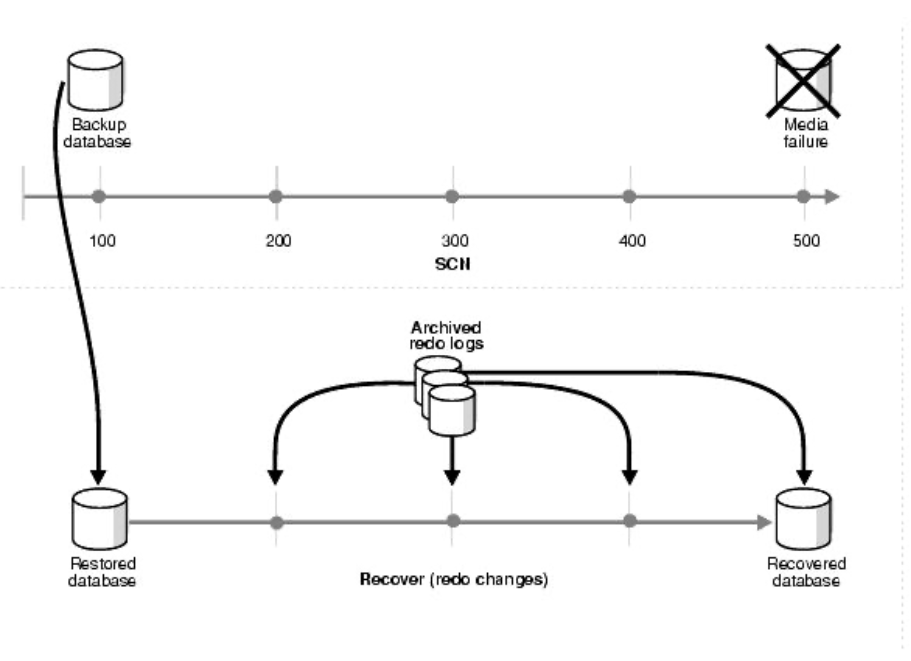
\includegraphics[width=.65\textwidth]{Content/images/backup/recovery.png}
    \caption{Für ein Recovery nimmt man einen Full-DB-Backup stand, und spielt auf diesem alle REDO-LOGS wieder ab, die seit diesem archiviert wurden.}
    \label{fig:backup:recovery}
\end{figure}

\subsection{Media-Recovery}

Media Recovery hilft gegen Media-Failure oder User-Errors. Dafür braucht man die gebackupten Control-Files, Data-Files, Archivierte Redo-Logs und die Redo-Logs der aktuell kaputten Datenbank. Dabei werden alle Redo-Logs, die nicht in der aktuell kaputten
Datenbank abgebildet sind abgespielt um den kompletten Stand der Datenbank wiederherzustellen. Media-Recoveries müssen manuell durchgeführt werden.

\subsection{Complete Recovery}

Die gesamten Daten vor dem Error werden wiederhergestellt. Es wird ein komplettes Backup genommen, und die seitdem aufgenommenen Inkrementellen-Backups werden darauf angewandt.

\subsection{Point-In-Time Recovery (Incomplete Recovery)}

Die Datenbank wird auf den Stand eines speziellen Punktes in der Vergangenheit gesetzt. Man kann auch einen einzelnen Tablespace Point-In-Time-Recoveren.

\subsection{Instance- und Crash-Recovery}

Diese Recovery-Arten werden von Oracle automatisch durchgeführt. Hierbei werden die - möglicherweise korrupten - Datenfiles wieder auf den Transaktionskonsistenten Stand, welcher vor dem Absturz vorhanden war gebracht.

\subsubsection{Instance-Recovery}

Dies ist der Fall, wenn ein Oracle-Cluster vorliegt. Bei diesem kann eine einzelne kaputte Instanz von den anderen - die noch funktionieren - recovered werden (Ähnlich wie bei einem Raid-FS)

\subsubsection{Crash-Recovery}

Dies ist der Fall, wenn alle Instanzen eines Clusters ausfallen.